\begin{figure*}
	\LARGE
	\begin{overpic}[width=\linewidth]{image/syn_qua.pdf}
        \put(5.6,4){\color{black}{\fontsize{8.7pt}{1pt}\selectfont $\text{0}^\circ$}}
        \put(5.3,17.4){\color{black}{\fontsize{8.7pt}{1pt}\selectfont $\text{20}^\circ$}}
        \put(5,36){\color{black}{\fontsize{9pt}{1pt}\selectfont GT}}
        \put(15,36){\color{black}{\fontsize{8pt}{1pt}\selectfont \nero}}
	    \put(26,36){\color{black}{\fontsize{8pt}{1pt}\selectfont \mvas}}        \put(35,36){\color{black}{\fontsize{8pt}{1pt}\selectfont \pandora}}        \put(47,36){\color{black}{\fontsize{8pt}{1pt}\selectfont \nersp}}        \put(55.5,36){\color{black}{\fontsize{8pt}{1pt}\selectfont \gs}}        \put(68.8,36){\color{black}{\fontsize{8pt}{1pt}\selectfont \dr}}        \put(80,36){\color{black}{\fontsize{8pt}{1pt}\selectfont \relight}}        \put(90,36){\color{black}{\fontsize{8pt}{1pt}\selectfont \polgs}}   
	    \put(16,1.7){\color{black}{\fontsize{9pt}{1pt}\selectfont $3.84^\circ$}}
	    \put(27.2,1.7){\color{black}{\fontsize{9pt}{1pt}\selectfont $8.73^\circ$}}
	    \put(38,1.7){\color{black}{\fontsize{9pt}{1pt}\selectfont $11.62^\circ$}}
	    \put(48.7,1.7){\color{black}{\fontsize{9pt}{1pt}\selectfont $10.14^\circ$}}	 
	    \put(59.8,1.7){\color{black}{\fontsize{9pt}{1pt}\selectfont $19.00^\circ$}}	
	    \put(70.8,1.7){\color{black}{\fontsize{9pt}{1pt}\selectfont $19.21^\circ$}}	
	    \put(81.8,1.7){\color{black}{\fontsize{9pt}{1pt}\selectfont $14.53^\circ$}}	
	    \put(92.8,1.7){\color{black}{\fontsize{9pt}{1pt}\selectfont $10.62^\circ$}}	
	    \put(4.4,1.7){\color{black}{\fontsize{8.7pt}{1pt}\selectfont MAE}}

	\end{overpic}
		   \vspace{-1.9em}
	\caption{Qualitative comparisons on surface normal estimation of {\sc Squirrel} in \smvp, where our 3DGS-based method can outperform existing methods based on the same representation and achieves comparable results with SDF-based methods such as \nersp and \pandora.
%		 The mean angular error map has shown in range of $0^\circ$ to $20^\circ$.
		%		 More results can be found in the supplementary material.
	}
	\label{fig:syn_normal}
\end{figure*}

\newcommand{\imgw}{0.28}
\begin{figure*}
	\huge
	\resizebox{1\linewidth}{!}{
		\begin{tabular}{@{}c@{}c@{}c@{}c@{}c@{}c@{}c@{}c@{}c@{}}
			Input & \nero & \mvas&	\pandora & \nersp &\gs  &\dr & \relight & \polgs \\  
			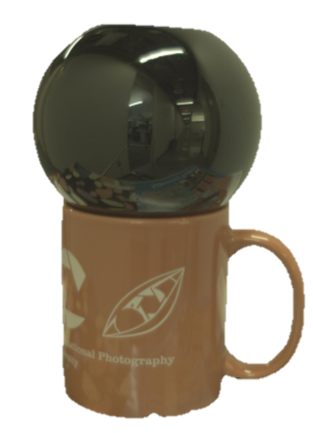
\includegraphics[width=\imgw\linewidth]{image/vase/gt.png}
			&
\includegraphics[width=\imgw\linewidth]{image/vase/shape_nero_crop.png}
			&
\includegraphics[width=\imgw\linewidth]{image/vase/shape_mvas_crop.png}
			&
\includegraphics[width=\imgw\linewidth]{image/vase/shape_pandora_crop.png}
			&
\includegraphics[width=\imgw\linewidth]{image/vase/shape_nersp_crop.png}
			&
\includegraphics[width=\imgw\linewidth]{image/vase/shape_gs_crop.png}
			&
\includegraphics[width=\imgw\linewidth]{image/vase/shape_dr_crop.png}
			&
\includegraphics[width=\imgw\linewidth]{image/vase/shape_re_crop.png}
			&
\includegraphics[width=\imgw\linewidth]{image/vase/shape_ours_crop.png}\\
			
			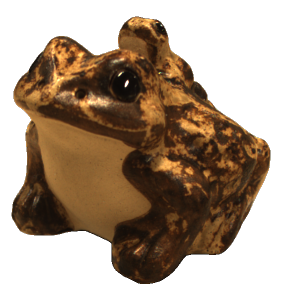
\includegraphics[width=\imgw\linewidth]{image/frog/0012.png}
			&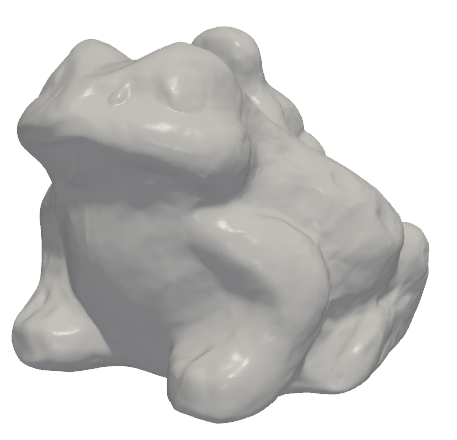
\includegraphics[width=\imgw\linewidth]{image/frog/shape_nero_crop.png}
			&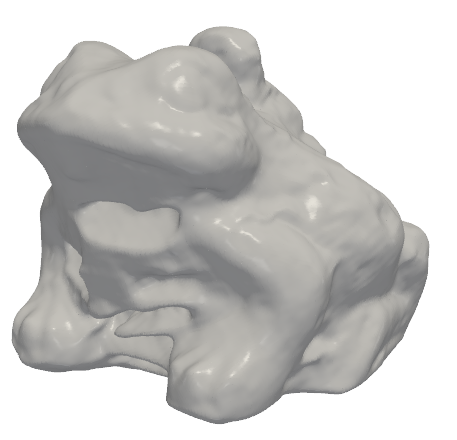
\includegraphics[width=\imgw\linewidth]{image/frog/shape_mvas_crop.png}
			&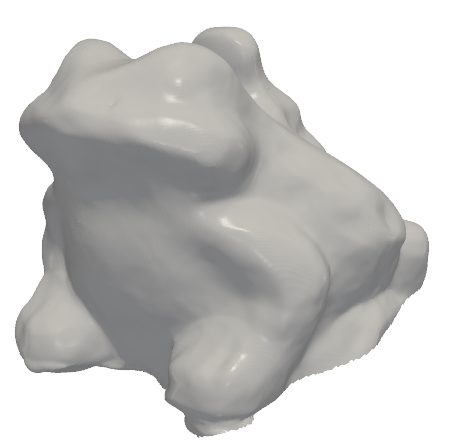
\includegraphics[width=\imgw\linewidth]{image/frog/shape_pandora_crop.png}
			&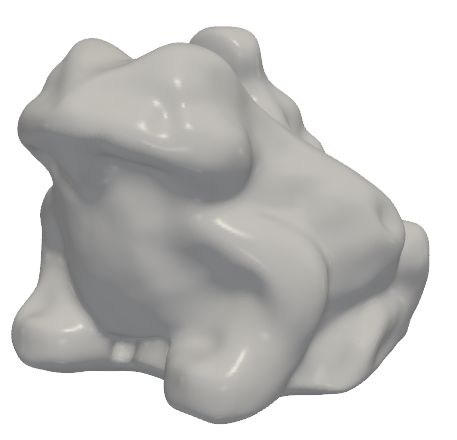
\includegraphics[width=\imgw\linewidth]{image/frog/shape_nersp_crop.png}
			
			&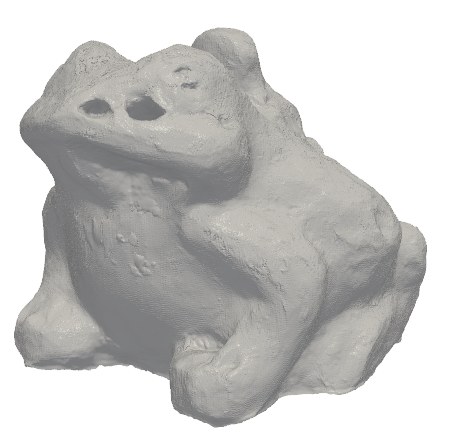
\includegraphics[width=\imgw\linewidth]{image/frog/shape_gs_crop.png}
			&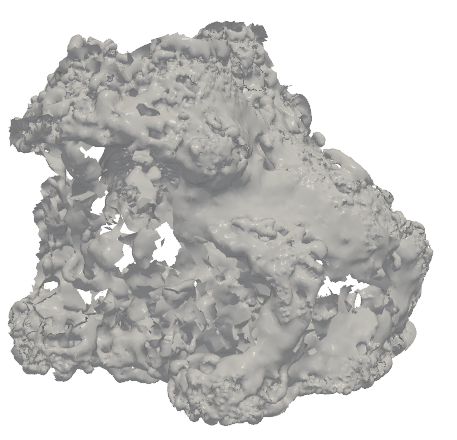
\includegraphics[width=\imgw\linewidth]{image/frog/shape_dr_crop.png}
			&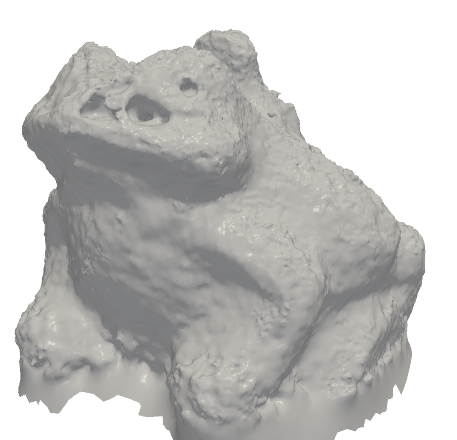
\includegraphics[width=\imgw\linewidth]{image/frog/shape_re_crop.png}
			&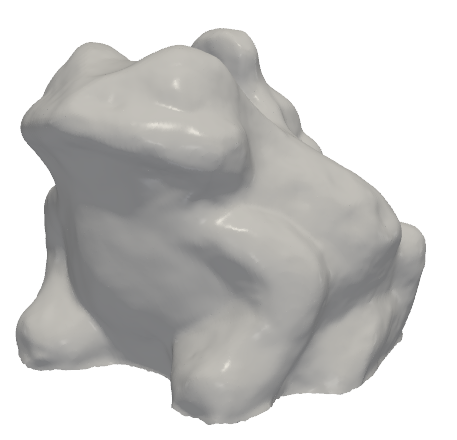
\includegraphics[width=\imgw\linewidth]{image/frog/shape_ours_crop.png}\\
			
		\end{tabular}
	}
	\caption{Qualitative comparison shape on \pandora and \rmvp, where \polgs produces similar quality of reconstruction mesh compared to SDF-based methods. }
	\label{fig:PANDORA-result}
    \vspace{-0.5em}
\end{figure*}
\section{Experiments}
To evaluate the performance of our method, we conduct these experiments: 1) Shape reconstruction 
on synthetic dataset, 2) Shape reconstruction on real-world dataset, 3) Radiance decomposition and 4) Ablation study of polarimetric constraint adding.
\vspace{-1.4em}\paragraph{Dataset}  We use three datasets to evaluate our method: the synthetic dataset \smvp, the real-world dataset \rmvp,
\pandora and \pisr, where \pandora can only be used for qualitative evaluation due to the lack of ground truth.
\vspace{-1.0em}
\paragraph{Baselines} 
We compare our method with state-of-the-art techniques, including SDF-based 
methods \nero, \mvas, \pandora, \nersp, and 3DGS methods \gs, \dr, and \relight. 
All of these methods, except \gs, can handle reflective surfaces. \mvas, \pandora and \nersp utilize 
polarimetric information to reconstruct shapes. Specifically, we do not add the normal prior in \gs among the whole experiments.
\vspace{-1em}
\paragraph{Evaluation metrics}
We use the Chamfer Distance (CD) to evaluate the shape recovery performance and 
the mean angular error (MAE) to evaluate the quality of surface normal estimations. 3DGS-based methods provide point cloud results and we use the Poisson surface reconstruction to generate the mesh for the evaluation.
\vspace{-1.2em}
\paragraph{Implementation details}
We conduct the experiments on an NVIDIA RTX 4090 GPU with 24GB memory. The training of our model is implemented in 
PyTorch 1.12.1 using the Adam optimizer. The specific learning rates of different components
in Gaussian kernels are set the same as \gs. We use the warm-up strategy to train the model, where adding the 
polarimetric information and deferred rendering after 1000 iterations.


\subsection{Reconstruction results on synthetic dataset}

In \fref{fig:syn_normal} and \Tref{table:shape_quantitative_value}, we compare the shape recovery performance of various methods on the \smvp dataset, which contains five objects with spatially varying and reflective properties. However, it is worth noting that SDF-based methods, such as \nero, \mvas, \pandora, and \nersp, outperform 3DGS methods in terms of surface representation. This advantage is largely due to their superior ability to model complex surface details. Among the 3DGS methods, \gs struggles with reflective surfaces, while \dr and \relight still has difficulty in representation of surface normal accurately.
In contrast, PolGS effectively leverages polarimetric information, significantly improving geometric surface performance. Due to the inadequate point cloud generation by other 3DGS methods, they fail to produce reasonable mesh results using Poisson surface reconstruction. Our method, however, achieves the lowest mean Chamfer Distance across the synthetic \smvp dataset, reinforcing the trends observed in surface normal estimations and confirming that our approach delivers the best performance among the 3DGS techniques.

\setlength{\aboverulesep}{-0.7pt}
\setlength{\belowrulesep}{-0pt}
\begin{table*}
	\caption{Comparisons on \smvp and \rmvp evaluated by mean angular error (MAE)~($\downarrow$) with degree and Chamfer distance (CD)~($\downarrow$) in millimeter (mm), respectively. 
	Best and second results in SDF-based and 3DGS-based methods (except PolGS w/o $\mathcal{L}_{pol}$) are highlighted as \colorbox[rgb]{1,0.7,0.7}{1st} and \colorbox[rgb]{1,1,0.4}{2nd}. The time consumed is shown on the far right side of the table.
	}
	\label{table:shape_quantitative_value}
	\vspace{-0.5em}
	\centering
	\LARGE
	\resizebox{\textwidth}{!}{
\begin{tabular}{lcccccccccc|cccccc|cc|c}
	\toprule
	& \multicolumn{10}{c|}{\smvp} & \multicolumn{6}{c|}{\rmvp}&&&
	
	\\
	\cmidrule{2-17}
	 & \multicolumn{2}{c}{\sc Hedgehog } & \multicolumn{2}{c}{\sc Squirrel} & \multicolumn{2}{c}{\sc Snail} & \multicolumn{2}{c}{\sc David} & \multicolumn{2}{c|}{\sc Dragon} & \multicolumn{2}{c}{\sc Shisa} & \multicolumn{2}{c}{\sc Frog} & \multicolumn{2}{c|}{\sc Dog}&\multicolumn{2}{c|}{\multirow{-2}{*}{Mean}}& \\
%	\cmidrule{2-19}
		\multicolumn{1}{c}{\multirow{-3}{*}{Method}} & MAE & CD & MAE & CD & MAE & CD & MAE & CD & MAE & CD & MAE & CD & MAE & CD & MAE & CD& MAE & CD& \multicolumn{1}{c}{\multirow{-3}{*}{time}}\\
	 \midrule
		 \pandora &9.41&9.50  &10.85& 5.88&8.08&10.97&14.75& 4.88&16.33& 4.78&
	12.93&11.29&15.86&7.88&20.11&10.19&13.54&8.17&10 h\\
	 
	 \nersp& 8.94&6.57 &8.23&  \colorbox[rgb]{1,1,0.4}{3.02}&5.56& \colorbox[rgb]{1,1,0.4}{3.72} &15.38&4.18 &15.30& 3.01&
	 10.79& \colorbox[rgb]{1,1,0.4}{7.39}& \colorbox[rgb]{1,1,0.4}{15.62}& \colorbox[rgb]{1,1,0.4}{6.68}& \colorbox[rgb]{1,0.7,0.7}{16.57}&  \colorbox[rgb]{1,0.7,0.7}{8.57} &12.05&\colorbox[rgb]{1,1,0.4}{5.39}&10 h
	 \\
	
	 \mvas &\colorbox[rgb]{1,1,0.4}{4.30}&\colorbox[rgb]{1,1,0.4}{4.22} & \colorbox[rgb]{1,1,0.4}{6.10}& 3.73 & \colorbox[rgb]{1,1,0.4}{3.30}& 7.87 & \colorbox[rgb]{1,1,0.4}{8.47}& \colorbox[rgb]{1,1,0.4}{3.21} &\colorbox[rgb]{1,0.7,0.7}{8.11}&  \colorbox[rgb]{1,1,0.4}{1.89}&  \colorbox[rgb]{1,1,0.4}{8.56}& 9.28& 17.63& 7.00&  \colorbox[rgb]{1,1,0.4}{16.65}& 8.76&\colorbox[rgb]{1,1,0.4}{9.01}&5.74&11 h\\
	 	
	 \nero &\colorbox[rgb]{1,0.7,0.7}{3.4}&\colorbox[rgb]{1,0.7,0.7}{3.69} & \colorbox[rgb]{1,0.7,0.7}{3.55}& \colorbox[rgb]{1,0.7,0.7}{1.86} & \colorbox[rgb]{1,0.7,0.7}{2.67}& \colorbox[rgb]{1,0.7,0.7}{3.71} &\colorbox[rgb]{1,0.7,0.7}{7.64}& \colorbox[rgb]{1,0.7,0.7}{2.88} &  \colorbox[rgb]{1,1,0.4}{8.12}&\colorbox[rgb]{1,0.7,0.7}{1.69}& \colorbox[rgb]{1,0.7,0.7}{8.41}& \colorbox[rgb]{1,0.7,0.7}{4.88}& \colorbox[rgb]{1,0.7,0.7}{15.29}& \colorbox[rgb]{1,0.7,0.7}{5.39}& 17.72& \colorbox[rgb]{1,1,0.4}{8.74}&\colorbox[rgb]{1,0.7,0.7}{8.27}&\colorbox[rgb]{1,0.7,0.7}{4.10}&8 h\\
	 
	 
    \midrule
    
    

    \dr &\colorbox[rgb]{1,1,0.4}{12.28}& 12.66&17.18& 11.20 &11.42& 20.7&20.56&7.91 &26.20 &  9.56  &19.53&15.87&17.08&27.67&24.85&11.00 &19.76&13.32& 0.2 h \\
    \relight &14.40& 19.84&\colorbox[rgb]{1,1,0.4}{15.41}&18.97 &\colorbox[rgb]{1,0.7,0.7}{9.08}& 19.04&\colorbox[rgb]{1,1,0.4}{15.47}& 13.47&\colorbox[rgb]{1,0.7,0.7}{17.65}&  10.96 &
	16.69&14.66&17.85&13.35&21.53 &12.24&\colorbox[rgb]{1,1,0.4}{15.89}&14.12& 0.4 h
	
	 \\
	\gs &16.50&\colorbox[rgb]{1,1,0.4}{8.82}&21.65& \colorbox[rgb]{1,1,0.4}{9.53}&19.05& \colorbox[rgb]{1,1,0.4}{14.04}&21.56& \colorbox[rgb]{1,1,0.4}{7.39}&\colorbox[rgb]{1,1,0.4}{21.41}&  \colorbox[rgb]{1,0.7,0.7}{6.98} &\colorbox[rgb]{1,1,0.4}{12.79}&\colorbox[rgb]{1,1,0.4}{9.09}&\colorbox[rgb]{1,1,0.4}{16.19}&\colorbox[rgb]{1,0.7,0.7}{7.01}&\colorbox[rgb]{1,1,0.4}{19.30}& \colorbox[rgb]{1,1,0.4}{9.56}&18.56&\colorbox[rgb]{1,1,0.4}{10.30}&0.2 h  \\
\polgs &\colorbox[rgb]{1,0.7,0.7}{10.83}&\colorbox[rgb]{1,0.7,0.7}{7.62}&\colorbox[rgb]{1,0.7,0.7}{11.42}& \colorbox[rgb]{1,0.7,0.7}{6.28}&\colorbox[rgb]{1,1,0.4}{9.64}&\colorbox[rgb]{1,0.7,0.7}{10.85}&\colorbox[rgb]{1,0.7,0.7}{13.99}& \colorbox[rgb]{1,0.7,0.7}{5.30}&24.23& \colorbox[rgb]{1,1,0.4}{7.61} &
	\colorbox[rgb]{1,0.7,0.7}{10.88}&\colorbox[rgb]{1,0.7,0.7}{7.76}&\colorbox[rgb]{1,0.7,0.7}{15.03}&\colorbox[rgb]{1,1,0.4}{7.48}&\colorbox[rgb]{1,0.7,0.7}{18.80}&\colorbox[rgb]{1,0.7,0.7}{7.71} &\colorbox[rgb]{1,0.7,0.7}{14.35}&\colorbox[rgb]{1,0.7,0.7}{7.57}&0.1 h\\
    \midrule
    PolGS w/o $\mathcal{L}_{pol}$ & 
    11.39&7.97&11.83&6.39&9.82&10.75&15.44&5.90&25.74&8.22&10.95&7.92&15.16&7.56&18.86&7.74&14.89&7.80&0.1 h\\
    
    
    \bottomrule
\end{tabular}	
}
\end{table*}


\subsection{Reconstruction results on real-world dataset}
We further evaluate the reconstruction performance on the \rmvp and \pandora datasets, with qualitative results illustrated in \fref{fig:PANDORA-result} and quantitative results detailed in \Tref{table:shape_quantitative_value}. In real-world scenarios, our method produces reconstructions that align more closely with SDF-based approaches, while significantly outperforming other 3DGS-based methods in terms of reconstruction quality. For example, in the {\sc Vase} case, our approach accurately estimates the shape of a ceramic surface in just $7$ minutes, achieving results closer to those generated by SDF-based methods. 
Additionally, the {\sc Frog} sample highlights our method's ability to reconstruct objects with rough glossy surfaces, showing the robustness and generalization capability of our method. These results collectively demonstrate the effectiveness of our approach in handling diverse real-world objects with varying surface properties. 



\begin{figure}
	\begin{overpic}[width=\linewidth, trim={0pt 0pt 0pt 0pt}]{image/env_2.pdf}
		
		\put(75,43){\color{black}{\fontsize{8pt}{1pt}\selectfont {\polgs}}}
		\put(10,43){\color{black}{\fontsize{8pt}{1pt}\selectfont {\pandora}}}
		\put(41.5,43){\color{black}{\fontsize{8pt}{1pt}\selectfont {\dr}}}
	\end{overpic}
	\vspace{-1.5em}
	\caption{Separation of diffuse and specular components with \pandora, \dr and \polgs.}
	\label{fig:env_compare}
	\vspace{-2em}
\end{figure}

%
\subsection{Comparison of radiance decomposition}
\Fref{fig:env_compare} presents a comparison of diffuse and specular component decomposition generated by \pandora, \dr, and \polgs. Here, \pandora utilizes the IDE~\cite{verbin2022ref} structure to produce environment map results, whereas \polgs adopts \dr's methods by employing a Cubemap encoder for the same purpose. 
Compared with \dr, \polgs leverages additional polarimetric information to effectively constrain and disambiguate diffuse and specular components. 
Notably, our results closely align with \pandora's, demonstrating improved radiance decomposition ability.


\begin{figure}
	\centering
\vspace{-1em}
	\begin{overpic}
		[width=\linewidth]{image/ablation.pdf}
		\put(12,1){\color{black}{\fontsize{9pt}{1pt}\selectfont GT normal}}
		\put(43,1){\color{black}{\fontsize{9pt}{1pt}\selectfont w/o $\mathcal{L}_{pol}$}}
		\put(80,1){\color{black}{\fontsize{9pt}{1pt}\selectfont w $\mathcal{L}_{pol}$}}
		\put(53,23){\color{black}{\fontsize{8pt}{1pt}\selectfont $14.57^\circ$}}
		\put(87,23){\color{black}{\fontsize{8pt}{1pt}\selectfont $12.51^\circ$}}
		\put(53,65){\color{black}{\fontsize{8pt}{1pt}\selectfont $10.29^\circ$}}
		\put(87,65){\color{black}{\fontsize{8pt}{1pt}\selectfont $9.71^\circ$}}
		\put(53,46){\color{black}{\fontsize{8pt}{1pt}\selectfont $10.24^\circ$}}
		\put(87,46){\color{black}{\fontsize{8pt}{1pt}\selectfont $9.73^\circ$}}
		\put(20,23){\color{black}{\fontsize{8pt}{1pt}\selectfont {\sc David}}}
		\put(20,46){\color{black}{\fontsize{8pt}{1pt}\selectfont {\sc Snail}}}
		\put(19,66){\color{black}{\fontsize{8pt}{1pt}\selectfont {\sc Hedgehog}}}
	\end{overpic}
		\vspace{-1.5em}
	\caption{Ablation study on  surface normal estimation with and without polarimetric information $\mathcal{L}_{pol}$. The MAE values are displayed on the top of each image. }
	\label{fig:ablation}
	\vspace{-1.5em}
\end{figure}



\subsection{Ablation study}\label{sec:ablation}

In this section, we conduct an ablation study to evaluate the contribution of polarimetric information to surface reconstruction. As shown in \Tref{table:shape_quantitative_value} and \fref{fig:ablation}, integrating $\mathcal{L}_{pol}$ consistently improves reconstruction accuracy across both synthetic and real-world datasets. The incorporation of $\mathcal{L}_{pol}$ particularly enhances geometric fidelity in challenging regions such as the {\sc Hedgehog}'s bottom and the {\sc Snail}'s back, where it effectively suppresses concave artifacts.

However, for texture-rich surfaces captured under dense views ($>$30 views), the existing photometric cues (RGB) provide sufficient constraints, leaving limited room for additional improvement from polarimetric information. This contrasts with texture-less surfaces like the {\sc David} statue, where $\mathcal{L}_{pol}$ contributes to reconstruction quality by providing additional geometric constraints.

\begin{figure}
	\vspace{-0.5em}
	\begin{overpic}[width=\linewidth, trim={0pt 0pt 0pt 0pt}]{image/rebuttal/ablation5.pdf}
		\put(17.5,44.5){\color{black}{\fontsize{7pt}{1pt}\selectfont GT}}
		\put(18,30){\color{black}{\fontsize{8pt}{1pt}\selectfont $s_2$}}
		\put(6.7,30){\color{black}{\fontsize{8pt}{1pt}\selectfont $s_1$}}     \put(6.5,44.5){\color{black}{\fontsize{8pt}{1pt}\selectfont $s_0$}}
		
		\put(1,13){\color{black}{\fontsize{8pt}{1pt}\selectfont $s_0$}}
		
		\put(35,13){\color{black}{\fontsize{8pt}{1pt}\selectfont $s_2$}}
		\put(18,13){\color{black}{\fontsize{8pt}{1pt}\selectfont $s_1$}}    
		\put(52,13){\color{black}{\fontsize{7pt}{1pt}\selectfont GT}}
		
		\put(28,19){\color{black}{\fontsize{8pt}{1pt}\selectfont w $\mathcal{L}_{pol}$}}
		\put(47,19){\color{black}{\fontsize{8pt}{1pt}\selectfont w/o $\mathcal{L}_{pol}$}}
		\put(67,19){\color{black}{\fontsize{8pt}{1pt}\selectfont w $\mathcal{L}_{pol}$}}
		\put(85,19){\color{black}{\fontsize{8pt}{1pt}\selectfont w/o $\mathcal{L}_{pol}$}}
		
		\put(35.5,45){\color{black}{\fontsize{7pt}{1pt}\selectfont $13.3^\circ$}}
		\put(55.5,45){\color{black}{\fontsize{7pt}{1pt}\selectfont $15.3^\circ$}}
		\put(75,45){\color{black}{\fontsize{7pt}{1pt}\selectfont $16.5^\circ$}}
		\put(94.8,45){\color{black}{\fontsize{7pt}{1pt}\selectfont $19.0^\circ$}}
		
		\put(37,49){\color{black}{\fontsize{8pt}{1pt}\selectfont {20 views}}}
		\put(75,49){\color{black}{\fontsize{8pt}{1pt}\selectfont {14 views}}}
		
		\put(71,0.5){\color{black}{\fontsize{8pt}{1pt}\selectfont w $\mathcal{L}_{pol}$}}
		\put(86,0.5){\color{black}{\fontsize{8pt}{1pt}\selectfont w/o $\mathcal{L}_{pol}$}}
		\put(85,13.8){\color{black}{\fontsize{7pt}{1pt}\selectfont $13.8^\circ$}}
		\put(67,13.8){\color{black}{\fontsize{7pt}{1pt}\selectfont $11.8^\circ$}}
		
	\end{overpic}
		\vspace{-1.5em}
	\caption{Stokes vectors can help surface normal reconstruction on texture-less surfaces.}
	\label{fig:r1}
	\vspace{-1.5em}
\end{figure}


\paragraph{Boosting on texture-less surfaces recovery with $\mathcal{L}_{pol}$}
To further validate the benefits of $\mathcal{L}_{pol}$ on texture-less surfaces, we conduct additional experiments using a real-world dataset from PISR~[{\color{iccvblue}5}], as shown in \fref{fig:r1}. While the RGB appearance lacks discernible texture, the polarization channels $s_1$ and $s_2$ exhibit meaningful variations that provide additional geometric cues for resolving shape ambiguities. The results show that both concave and convex surface distortions are more accurately reconstructed when $\mathcal{L}_{pol}$ is employed. Moreover, as the number of input views decreases, the advantages of incorporating polarization become even more evident. This demonstrates the unique value of polarimetric information in challenging scenarios where conventional RGB inputs offer limited constraints.



